\documentclass[12pt,a4paper]{article}

\usepackage{amsmath,amssymb}
\usepackage{graphicx}
\usepackage{hyperref}
\usepackage{natbib}
\usepackage{geometry}
\usepackage{booktabs}
\usepackage{xcolor}
\usepackage{setspace}

\geometry{margin=1in}
\onehalfspacing

\hypersetup{
  colorlinks=true,
  linkcolor=black,
  citecolor=black,
  urlcolor=black
}

% ─────────────────────────────────────────────────────────────────────────────
\title{\textbf{The Two Faces of Time}\\
\large Coordinate Time, Proper Time, and Accumulated Decoherence}

\author{Heath W.\ Mahaffey\\
\small Independent Researcher, Entiat, WA 98822, USA\\
\small \texttt{hmahaffeyges@gmail.com}\\
\small \texttt{https://github.com/hmahaffeyges/IAM-Validation}}

\date{March 2026; revised October 2026\\
\small Zenodo DOI:
\href{https://doi.org/10.5281/zenodo.18702042}{10.5281/zenodo.18702042}}
% ─────────────────────────────────────────────────────────────────────────────

\begin{document}
\maketitle

% ─────────────────────────────────────────────────────────────────────────────
\begin{abstract}
Time enters physics in more than one role. The Machian relational framework
\citep{BarbourBertotti1982} showed that coordinate time is a redundant label on
the spacetime manifold. We distinguish three quantities that are often treated
interchangeably: (i)~coordinate time, a label with no preferred direction and no
accumulation; (ii)~proper time $\tau$, the geometric path length along a
worldline, which does not by itself distinguish past from future; and
(iii)~accumulated decoherence, measured in the Informational Actualization Model
(IAM) by the activation function $E(a)=\exp(1-1/a)$: thermodynamic, irreversible,
and carried only by massive particles. Photons travel null geodesics, $d\tau=0$:
they accumulate neither proper time nor decoherence. Massive particles accumulate
both and constitute the matter sector. The sector separation follows from the
causal structure of the manifold combined with the thermodynamic cost of
irreversible decoherence on timelike worldlines. Within this picture the arrow of
time is set by the irreversibility of each decoherence event, each of which carries
a minimum cost $k_BT\ln2$ per bit \citep{Landauer1961}; $E(a)$ is monotonically
increasing. We show how the distinction bears on the Hubble tension and how it sits
within shape dynamics.
\end{abstract}

\noindent\textbf{Keywords:} time; accumulated decoherence; Machian relationism; arrow of
time; electroweak symmetry breaking; gravitational decoherence; sector
separation; Informational Actualization Model

% ─────────────────────────────────────────────────────────────────────────────
\section{Two Faces}
\label{sec:twofaces}
% ─────────────────────────────────────────────────────────────────────────────

Time is two-faced.

Barbour identified the first face in 1982 with the Machian relational
framework: coordinate time is redundant, a label on a dimension, not a
river carrying us forward~\citep{BarbourBertotti1982}. That result
has shaped how foundational questions about time are posed.

The second face concerns irreversibility. Is every temporal quantity equally
redundant? We argue that one is not: the accumulated count of irreversible
decoherence events on a worldline has a physical carrier and a direction, and the
relational framework accommodates it naturally.

\section{Three Quantities Worth Distinguishing}
\label{sec:threequantities}
% ─────────────────────────────────────────────────────────────────────────────

Time appears in physical theory in at least three distinct roles that
are worth distinguishing carefully. The differences between them are
not merely terminological.

\subsection{Coordinate time: the map}

Coordinate time, $t$ or the scale factor $a$, is a label on the
spacetime manifold. It assigns a number to each event. It does not require
anything to happen. It does not require worldlines to exist, mass to be
present, or irreversible processes to occur. The manifold exists with its
coordinate structure whether or not any event within it is irreversible.

Barbour's central insight~\citep{BarbourBertotti1982,Barbour1994} is that
this coordinate has no privileged status. It is redundant as a fundamental
concept. The relational framework constructs dynamics from configurations
alone, without reference to an external temporal parameter.
Coordinate time is the map. It is not the territory.

\subsection{Proper time: path length on the map}

Proper time $\tau$ is the geometric path length along a worldline:
\begin{equation}
\tau = \int \sqrt{-g_{\mu\nu}\,dx^\mu dx^\nu}.
\end{equation}
It is still a geometric quantity, a property of the spacetime manifold
measured along a particular path. A clock measures proper time. It tells
you how far you have traveled on the map.

Critically, proper time is reversible in principle. In a universe with
time-reversal symmetric laws, a worldline running forward and backward in
coordinate time accumulates $\tau$ in both directions. Proper time
distinguishes clocks from one another but does not, by itself, distinguish
past from future.

For null geodesics, photons, $d\tau = 0$ identically. Photons plot on
the manifold but accumulate zero proper time. This is not an approximation.
It is the definition of a null geodesic.

\subsection{Accumulated decoherence: the record}

Accumulated decoherence is different from both coordinate time and proper
time. It is not a geometric quantity. It is thermodynamic.

It counts the irreversible quantum-to-classical transitions on a worldline, the
decoherence events that write classical information on the cosmic horizon at a
Landauer cost $k_BT\ln 2$ per bit~\citep{Landauer1961}. It requires:
\begin{enumerate}
\item massive particles on timelike worldlines ($d\tau > 0$);
\item irreversible quantum-to-classical transitions (gravitational decoherence).
\end{enumerate}
Massive particles exist from electroweak symmetry breaking ($T\approx100$ GeV,
$t\approx10^{-11}$~s), when the $W$, $Z$ and the charged fermions acquire mass
\citep{mahaffey2026higgs}. The irreversibility itself does not depend on CP
violation: decoherence and entropy production are irreversible for any
interaction. $E(a)$ is negligible for most of cosmic history
($E(z=10)=4.5\times10^{-5}$) and grows as structure forms.

The geometric and thermodynamic descriptions are shown in Figure~\ref{fig:twofaces}. The same
worldline admits a geometric and a thermodynamic description.

\begin{figure}[htbp]
\centering
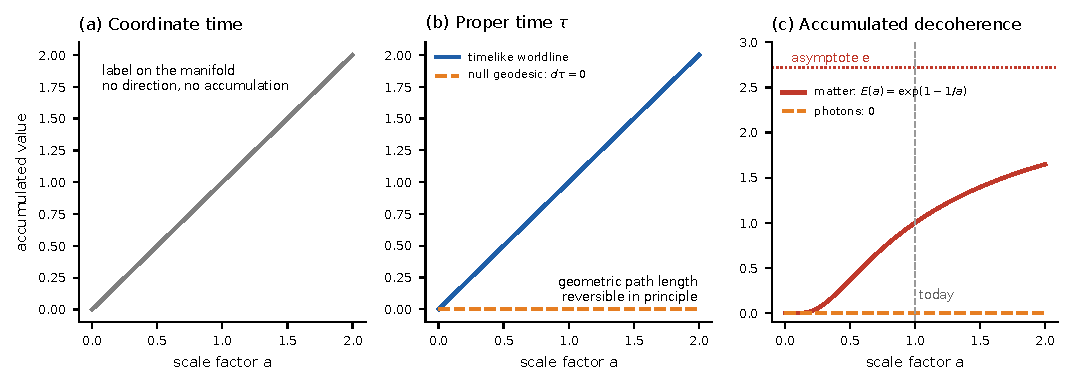
\includegraphics[width=0.85\textwidth]{two_faces_of_time_figure.pdf}
\caption{The two faces of time. Panel~(a): geometric quantities,
coordinate time (redundant label, \citealt{BarbourBertotti1982}) and proper
time $\tau$ (path length along worldline). Photons plot on the manifold but
accumulate neither. Panel~(b): accumulated decoherence, $E(a) = \exp(1-1/a)$, a
thermodynamic quantity distinct from both: irreversible and carried by massive
particles only. The matter sector and photon sector are separated by construction.}
\label{fig:twofaces}
\end{figure}

% ─────────────────────────────────────────────────────────────────────────────
\section{The Second Face: Accumulated Decoherence}
\label{sec:decoherence}
% ─────────────────────────────────────────────────────────────────────────────

\subsection{The activation function}

Within the Informational Actualization Model
(IAM,~\citealt{mahaffey2026}), accumulated decoherence is measured by the
activation function:
\begin{equation}
E(a) = \exp\!\left(1 - \frac{1}{a}\right),
\label{eq:Ea}
\end{equation}
where $a$ is the cosmological scale factor normalized to unity today.

The properties of $E(a)$ follow directly from its physical interpretation:
\begin{itemize}
\item $E(a) \to 0$ as $a \to 0$: negligible in the early universe.
\item $E(1) = 1$: normalized to today.
\item $E(a) \to e$ as $a \to \infty$: a finite asymptote, approached but never
attained.
\item $dE/da > 0$ always: monotonically increasing, one direction only.
\end{itemize}

The monotonic increase is not imposed. It follows from the irreversibility
of each decoherence event. Each bit written on the horizon cannot be
unwritten. The record only accumulates. This is the arrow of time, not
statistical, not initial-condition-dependent, but thermodynamically
necessary.

\subsection{Photons do not accumulate decoherence}

Photons travel null geodesics. $d\tau = 0$ by construction. No proper time
accumulates. No gravitational decoherence occurs; decoherence requires
nonzero proper time on a timelike worldline. Therefore:
\begin{equation}
E(a)\big|_{\text{photon}} \equiv 0.
\end{equation}

This is the physical basis for the sector split. Photons interact with the
spacetime geometry; they are bent by gravity, redshifted by expansion,
but they add nothing to $E(a)$. The modification to gravitational
dynamics that $E(a)$ produces applies exclusively to the matter sector.

\subsection{The Machian framework already knew this}

The relational framework insists that physics be built from observable
relations between things. Coordinate time fails this test, it is not
directly observable. Proper time passes: clocks measure it. Accumulated
decoherence passes as well, and it is the temporal quantity that distinguishes
past from future through a physical mechanism rather than a statistical
assumption.

Mach's criterion, ``time is an abstraction at which we arrive through the changes
of things'', selects physical change over coordinate time. Not all changes are
equal: reversible changes leave $E(a)$ unchanged; only irreversible decoherence
events, each paying its Landauer cost, advance it.

\section{What the Sector Split Implies}
\label{sec:sectorsplit}
% ─────────────────────────────────────────────────────────────────────────────

The distinction between the geometric and thermodynamic quantities has an immediate
observational consequence that may help clarify a persistent tension
in cosmological observations.

The CMB measurement of $H_0$ uses photons emitted at last scattering,
traveling null geodesics for 13.8 billion years. The entire measurement is
geometric. No proper time accumulated and no decoherence recorded. It reads the
geometry. $H_0^{\text{photon}} = 67.16$~km\,s$^{-1}$\,Mpc$^{-1}$ is what the
manifold says about its own expansion rate~\citep{PlanckCollaboration2020}.

The local distance ladder uses Cepheids, Type~Ia supernovae, and TRGB
stars, massive objects on timelike worldlines that have accumulated
decoherence for billions of years. It reads the matter sector.
$H_0^{\text{matter}} = 72.26$~km\,s$^{-1}$\,Mpc$^{-1}$ is what the
matter sector says about its own expansion
rate~\citep{Riess2022,mahaffey2026obs}.

Within this framework, these are not necessarily two measurements of the
same quantity. They may be measurements of two distinct quantities,
one geometric and one thermodynamic, that a purely geometric treatment
does not distinguish. The Hubble tension is consistent with the sector
split, and the predicted values are derived from first principles with
zero free parameters beyond $\Lambda$CDM.

The predicted split follows from a single coupling constant derived from
the virial theorem:
\begin{equation}
\beta_m = \frac{\Omega_m}{2} = 0.15765,
\label{eq:betam}
\end{equation}
with zero free parameters beyond $\Lambda$CDM~\citep{mahaffey2026}.

% ─────────────────────────────────────────────────────────────────────────────
\section{The Relational Framework and Shape Dynamics}
\label{sec:shapedynamics}
% ─────────────────────────────────────────────────────────────────────────────

Shape dynamics~\citep{Barbour2011,BarbourKoslowskiMercati2014} replaces
four-dimensional spacetime refoliation invariance with three-dimensional
conformal invariance. The universe is described by the evolution of shape,  the relational configuration of matter, without reference to
absolute scale or absolute time.

IAM is compatible with this framework at every level. IAM does not modify
the background geometry. It does not alter the Friedmann equations. It
operates at the perturbation level, adding a single Hubble friction term
to the matter perturbation equations:
\begin{equation}
\ddot{\delta}_m + 2H\dot{\delta}_m - \frac{3}{2}\Omega_m H^2 \mu(a)\,\delta_m = 0,
\end{equation}
where
\begin{equation}
\mu(a) = \frac{H^2_{\Lambda\text{CDM}}}{H^2_{\Lambda\text{CDM}} + \beta_m E(a)} < 1.
\end{equation}

The geometric arena (shape space, the relational configuration) is untouched.
Accumulated decoherence is what happens on the worldlines \textit{within} that
arena; it does not modify the arena itself. Shape dynamics asks what the
universe's configuration is; IAM asks how much irreversible information the matter
sector has produced in reaching it. The two questions are complementary.

\section{An Open Question}
\label{sec:openquestion}
% ─────────────────────────────────────────────────────────────────────────────

Electroweak symmetry breaking selects one point of the degenerate Higgs vacuum
manifold. Is that selection itself the first gravitational-scale decoherence event,
with its own Landauer cost at the transition temperature? This remains an open question~\citep{mahaffey2026higgs}.


% ─────────────────────────────────────────────────────────────────────────────
\section{Repository}
\label{sec:repository}
% ─────────────────────────────────────────────────────────────────────────────

The complete thermodynamic derivation is developed in the IAM theory
paper~\citep{mahaffey2026}. The full collection of papers addressing
observational consequences, foundational extensions, open problems, and
future predictions is available in the documents folder of the repository
at \url{https://github.com/hmahaffeyges/IAM-Validation}. Follow whichever
thread interests you.

% ─────────────────────────────────────────────────────────────────────────────
\section*{Acknowledgments}
% ─────────────────────────────────────────────────────────────────────────────

The debt to Jacobson~\citeyearpar{Jacobson1995},
Cai and Kim~\citeyearpar{CaiKim2005}, and
Barbour and Bertotti~\citeyearpar{BarbourBertotti1982} is explicit
throughout. This work builds directly on their foundational contributions.

% ─────────────────────────────────────────────────────────────────────────────
\bibliographystyle{plainnat}
\begin{thebibliography}{99}

\bibitem[Barbour \& Bertotti(1982)]{BarbourBertotti1982}
Barbour, J.~B., \& Bertotti, B.\ 1982, Proceedings of the Royal Society
of London A, 382, 295

\bibitem[Barbour(1994)]{Barbour1994}
Barbour, J.~B.\ 1994, Classical and Quantum Gravity, 11, 2853

\bibitem[Barbour(2011)]{Barbour2011}
Barbour, J.~B.\ 2011, arXiv:1105.0183

\bibitem[Barbour, Koslowski \& Mercati(2014)]{BarbourKoslowskiMercati2014}
Barbour, J.~B., Koslowski, T., \& Mercati, F.\ 2014, Physical Review
Letters, 113, 181101

\bibitem[Cai \& Kim(2005)]{CaiKim2005}
Cai, R.-G., \& Kim, S.~P.\ 2005, Journal of High Energy Physics, 02, 050

\bibitem[Jacobson(1995)]{Jacobson1995}
Jacobson, T.\ 1995, Physical Review Letters, 75, 1260

\bibitem[Landauer(1961)]{Landauer1961}
Landauer, R.\ 1961, IBM Journal of Research and Development, 5, 183

\bibitem[Mahaffey(2026a)]{mahaffey2026}
Mahaffey, H.~W.\ 2026a, Horizon Thermodynamics and Gravitational
Decoherence as the Origin of $\mu < 1$, $\Sigma = 1$,
Zenodo DOI: 10.5281/zenodo.18702042

\bibitem[Mahaffey(2026b)]{mahaffey2026obs}
Mahaffey, H.~W.\ 2026b, Dual-Sector Perturbation Cosmology: CAMB
Implementation and Validation, Zenodo DOI: 10.5281/zenodo.18702042

\bibitem[Mahaffey(2026c)]{mahaffey2026higgs}
Mahaffey, H.~W.\ 2026c, Electroweak Symmetry Breaking and the Matter Sector,
Zenodo DOI: 10.5281/zenodo.18702042

\bibitem[Planck Collaboration(2020)]{PlanckCollaboration2020}
Planck Collaboration\ 2020, Astronomy \& Astrophysics, 641, A6

\bibitem[Riess et al.(2022)]{Riess2022}
Riess, A.~G., et al.\ 2022, The Astrophysical Journal Letters, 934, L7

\bibitem[Sakharov(1967)]{Sakharov1967}
Sakharov, A.~D.\ 1967, JETP Letters, 5, 24

\end{thebibliography}

\end{document}
